\begin{figure}[ht]
\centering

	\vbox{ 
		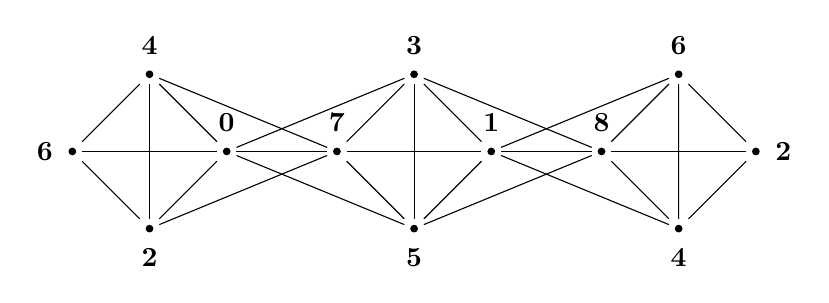
\begin{tikzpicture}[scale=0.7]

		\node[label=left: $\bf{ 6}$] (v1) at ( 0.0, 0.0) {};\fill (v1) circle (2pt);
		\node[label=above:$\bf{ 4}$] (v2) at ( 1.4, 1.4) {};\fill (v2) circle (2pt);
		\node[label=above:$\bf{ 0}$] (v3) at ( 2.8, 0.0) {};\fill (v3) circle (2pt);
		\node[label=below:$\bf{ 2}$] (v4) at ( 1.4,-1.4) {};\fill (v4) circle (2pt);
		
		\node[label=above:$\bf{ 7}$] (v5) at ( 4.8, 0.0) {};\fill (v5) circle (2pt);
		\node[label=above:$\bf{ 3}$] (v6) at ( 6.2, 1.4) {};\fill (v6) circle (2pt);
		\node[label=above:$\bf{ 1}$] (v7) at ( 7.6, 0.0) {};\fill (v7) circle (2pt);
		\node[label=below:$\bf{ 5}$] (v8) at ( 6.2,-1.4) {};\fill (v8) circle (2pt);
	
		\node[label=above:$\bf{ 8}$] (v9)  at ( 9.6, 0.0) {};\fill (v9) circle (2pt);
		\node[label=above:$\bf{ 6}$] (v10) at ( 11.0, 1.4) {};\fill (v10) circle (2pt);
		\node[label=right:$\bf{ 2}$] (v11) at (12.4, 0.0) {};\fill (v11) circle (2pt);
		\node[label=below:$\bf{ 4}$] (v12) at ( 11.0,-1.4) {};\fill (v12) circle (2pt);

		\draw[-] (v1) to (v2); \draw[-]  (v1) to (v3); \draw[-]  (v1) to (v4);
		\draw[-] (v2) to (v3); \draw[-]  (v2) to (v4);
		\draw[-] (v3) to (v4);
		
		\draw[-] (v2) to (v5);
		\draw[-] (v3) to (v5);		
		\draw[-] (v4) to (v5);
		
    	\draw[-] (v6) to (v3);
		\draw[-] (v5) to (v3);		
		\draw[-] (v8) to (v3);
				
		\draw[-] (v5) to (v6); \draw[-]  (v5) to (v7); \draw[-]  (v5) to (v8);
		\draw[-] (v6) to (v7); \draw[-]  (v6) to (v8);
		\draw[-] (v7) to (v8);

		\draw[-] (v6) to (v9);
		\draw[-] (v7) to (v9);		
		\draw[-] (v8) to (v9);
		
    	\draw[-] (v10) to (v7);
		\draw[-] (v9) to (v7);		
		\draw[-] (v12) to (v7);
		
		\draw[-] (v9) to (v10); \draw[-] (v9) to (v11); \draw[-] (v9) to (v12);
		\draw[-] (v10) to (v11); \draw[-]  (v10) to (v12);
		\draw[-] (v11) to (v12);
		
	\end{tikzpicture}
	}
\caption{Example of the $L(2,1)-$labeling problem with $\lambda_{2,1}(G) = 8$.}
\label{fig:1}
\end{figure}